\documentclass[12pt]{article}
\usepackage{hyperref}
\usepackage[authoryear, round,sort,comma,numbers]{natbib}
\usepackage{times}
\usepackage{color}
\usepackage{apalike}
\usepackage{graphicx}
\usepackage{authblk}
\usepackage{amsmath}



%\usepackage[maxbibnames=99]{biblatex}
%\usepackage{setspace}
%\usepackage{geometry}
\usepackage[font={sf,small}]{caption}
%\usepackage{setspace}
%\usepackage{geometry}
%\usepackage{hyperref}
%\hypersetup{
%    colorlinks,
%    citecolor=black,
%    filecolor=black,
%    linkcolor=black,
%    urlcolor=black
%}
%\geometry{letterpaper}

\usepackage{amssymb}
%\usepackage{epstopdf}
\usepackage{float}
%\DeclareGraphicsRule{.tif}{png}{.png}{`convert #1 `dirname #1`/`basename #1 .tif`.png}

\newcommand{\specialcell}[2][c]{%
	\begin{tabular}[#1]{@{}c@{}}#2\end{tabular}}
\setlength{\textheight}{9.3in}
\setlength{\textwidth}{7in}
\setlength{\footskip}{0.5in}
\setlength{\topmargin}{-0.5in}
\setlength{\headheight}{0.2in}
\setlength{\headsep}{0in}
\setlength{\parindent}{1pc}
\setlength{\oddsidemargin}{-0.25in}
\setlength{\evensidemargin}{-0.25in}
\renewcommand{\baselinestretch}{1.5}


\title{Any way the brain blows?  What is the nature of decision noise in random exploration?}

\author[1]{Siyu Wang}
\author[1,2]{Robert C. Wilson}


\affil[1]{Department of Psychology, University of Arizona, Tucson AZ USA}
\affil[2]{Cognitive Science Program, University of Arizona, Tucson AZ USA}


\date{\today}

\begin{document}
	\maketitle
	
	\newpage
	
	
	\begin{figure}[H]
		\begin{center}
			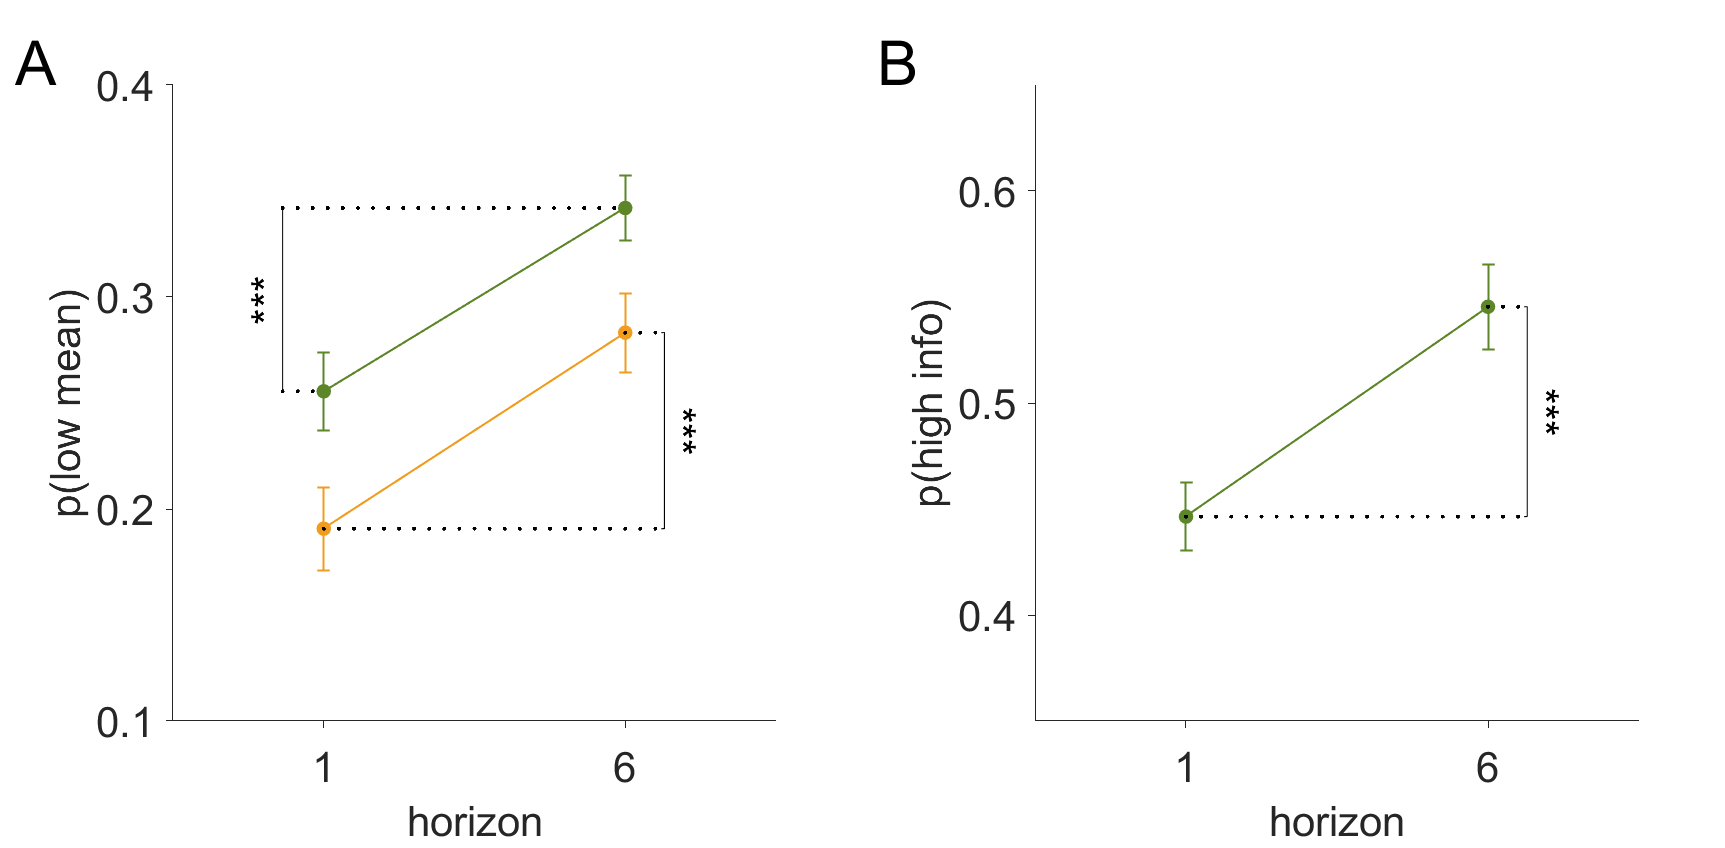
\includegraphics[width=\textwidth]{figures/line_modelfree.png}
			\caption{Both directed and random exploration increase with horizon. Choice inconsistency also increases with horizon for both [1 3] and [2 2] conditions.}
			\label{fig:modelfree2}
		\end{center}
	\end{figure}

	\begin{figure}[H]
		\begin{center}
			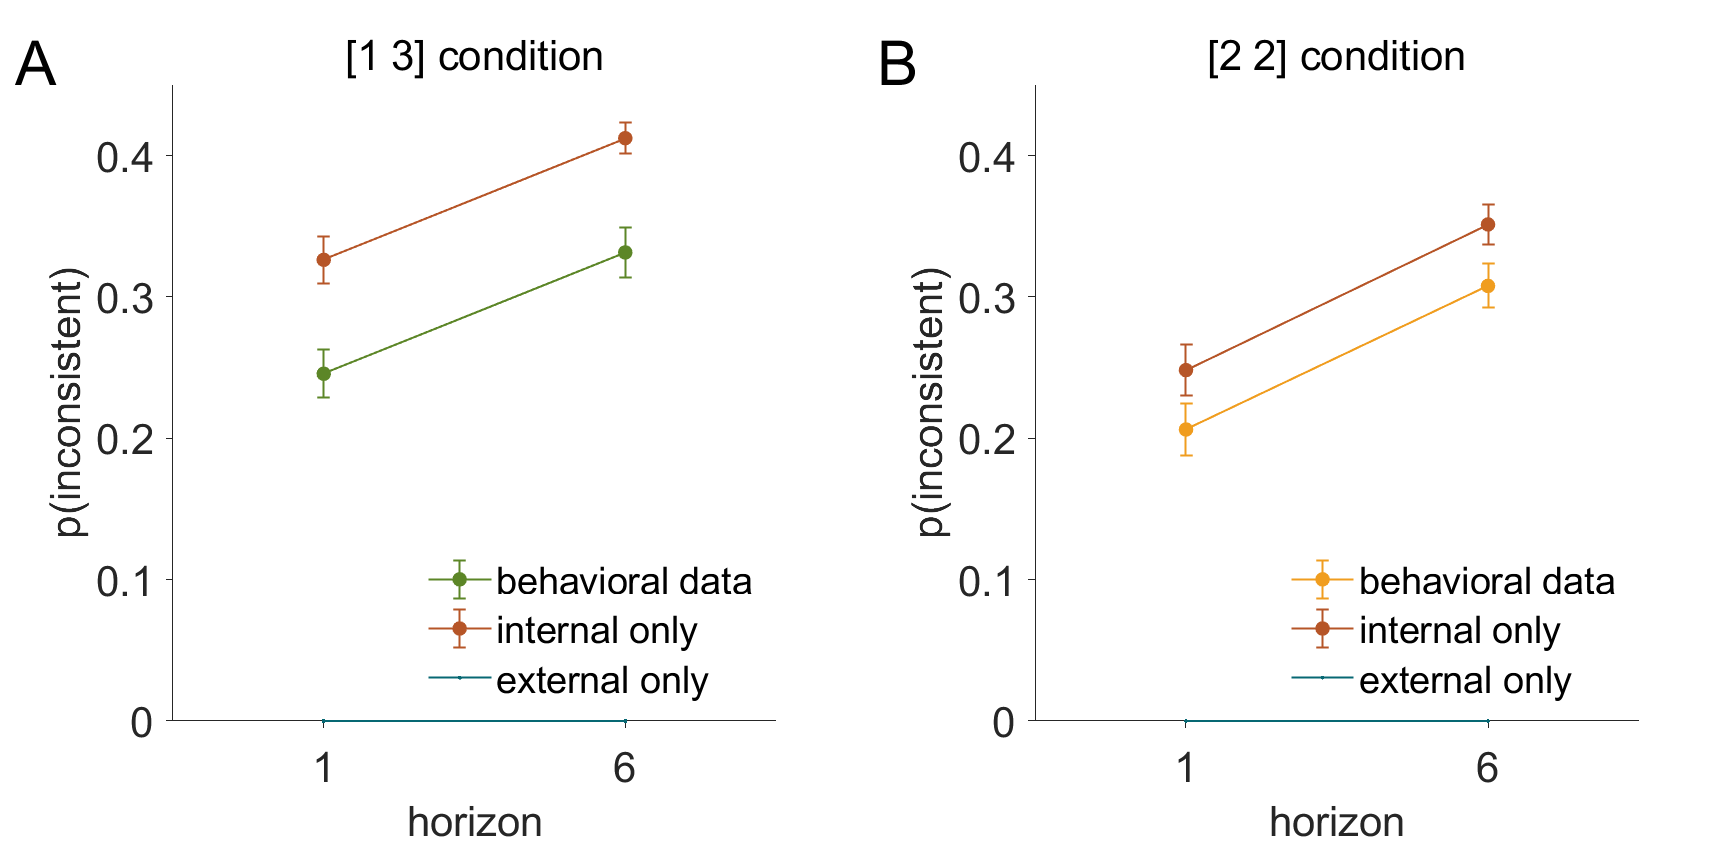
\includegraphics[width=\textwidth]{figures/theory_da_info.png}
			\caption[Both external and internal noise contribute to the choice variability in random exploration]{Both external and internal noise contribute to the choice variability in random exploration. For both [1 3] and [2 2] condition, there is a significant difference between people's behavior and predicted choice inconsistency assuming that only external noise exists where people should behave identically in repeated games. Also, there is a significant difference between people's behavior and predicted choice inconsistency assuming that only internal noise exists where people treat repeated games independently. }
			\label{fig:mf22}
		\end{center}
	\end{figure}
	\newpage
	\begin{figure}[H]
		\begin{center}
			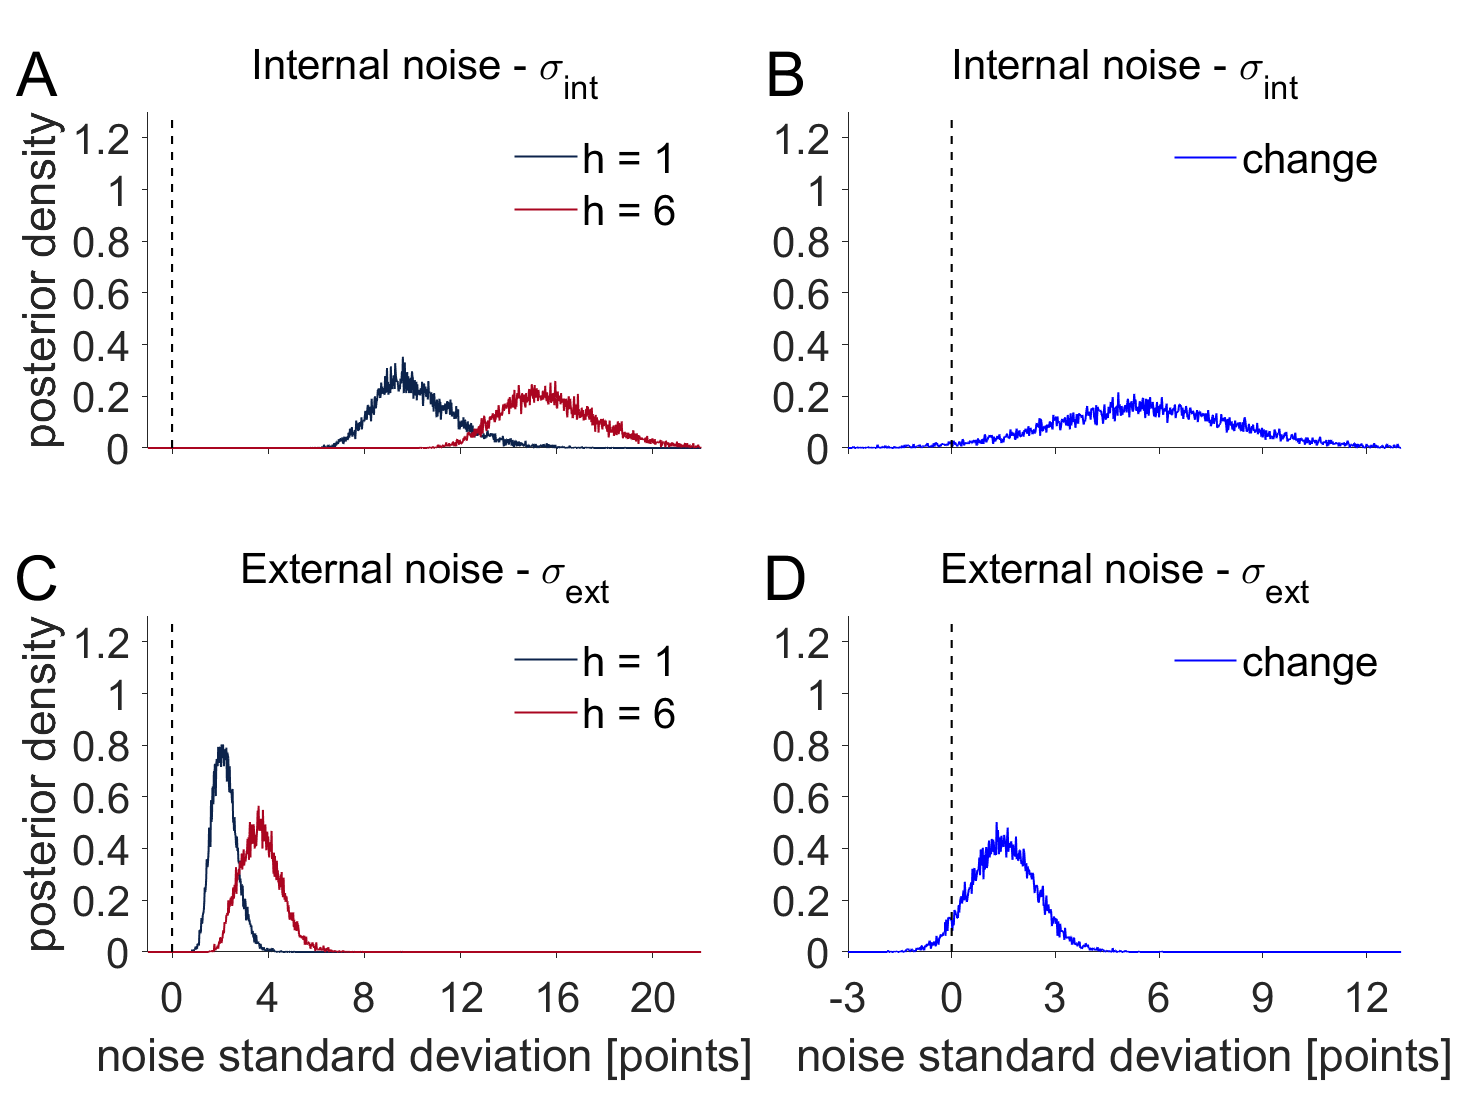
\includegraphics[width=1\textwidth]{figures/hyperprior.png}
			\caption[Posterior distributions over the group-level noise standard deviation of the external and internal noise variance.]{Posterior distributions over the group-level means of the external and internal noise standard deviation. Both internal and external noises are nonzero, and internal noise has a much greater magnitude. Posterior distributions over the group-level means of the change of external and internal noise standard deviation. Internal noise increases significantly with horizon, external noise increases with horizon as well.}
			%COMBINE FIGURES 4 AND 5, USE SEPARATE PANELS FOR EACH ONE, REMOVE INCORRECT RED SHADED REGION ON TOP PANEL OF FIGURE 5, Y-AXIS CAN BE LABELED 'posterior density' X-AXIS IS 'noise standard deviation [points]'
			\label{fig:mb12}
		\end{center}
	\end{figure}
	
	%\bibliographystyle{plainnat}
	%\bibliographystyle{unsrt}
	%\bibliography{Refs/refs}
	
	% add the Bibliography to the Table of Contents
	%\cleardoublepage
	%\ifdefined\phantomsection
	%\phantomsection  % makes hyperref recognize this section properly for pdf link
	%\else
	%\fi
	%\addcontentsline{toc}{chapter}{Bibliography}

\end{document}
